En esta sección se analizará la estabilidad del lazo de tensión en \texttt{LTSpice}, para lo cual se utilizó el circuito de la \autoref{fig:circuito LT}.

\begin{figure}[H]
    \centering
    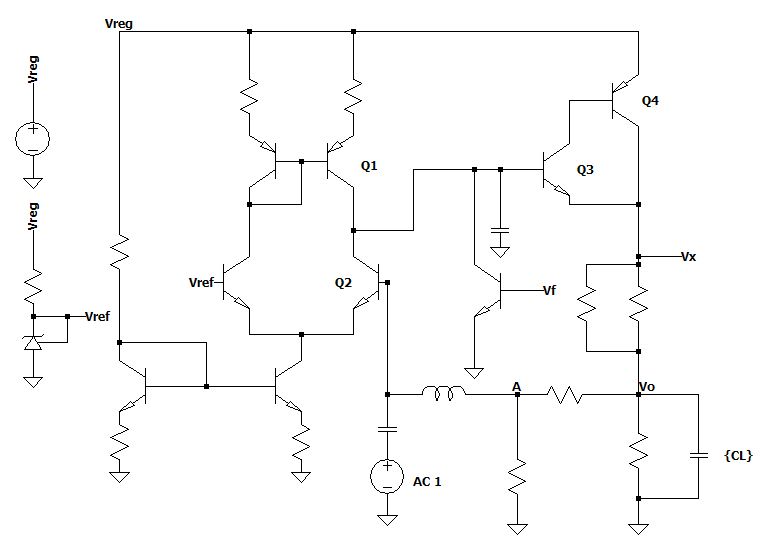
\includegraphics[width=0.9\linewidth]{img/Lazo de tensión/Circuito LT.png}
    \caption{Circuito utilizado para medir el lazo de tensión}
    \label{fig:circuito LT}
\end{figure}

En el mismo, la fuente de tensión \texttt{AC 1} funciona como la entrada a una de las terminales del par diferencial y se mide la salida del realimentador f (nodo A), obteniendo así la transferencia $L = a\cdot f$. El capacitor unido a la base de Q3 es el capacitor de compensación, que en principio es de 0 F.

Como puede verse en las directivas, la capacidad $C_L$ puede tomar 2 valores, \SI{1}{\micro \farad} y \SI{15}{\micro \farad}. Además, la carga puede variar entre \SI{3,4}{\ohm} y \SI{50}{\ohm}, por lo que se tienen 4 circuitos distintos para compensar. Para hacer la tarea más simple se optó por compensar el circuito con el peor margen de fase, lo que compensaría a todos a la vez. Luego de un breve análisis de obtuvo que el peor caso se da para la combinación $R_L = 50 \Omega$ y $C_L = \SI{1}{\micro \farad}$, cuyo diagrama de Bode se muestra el la \autoref{fig:LT sin compensar}

\begin{figure}[H]
    \centering
    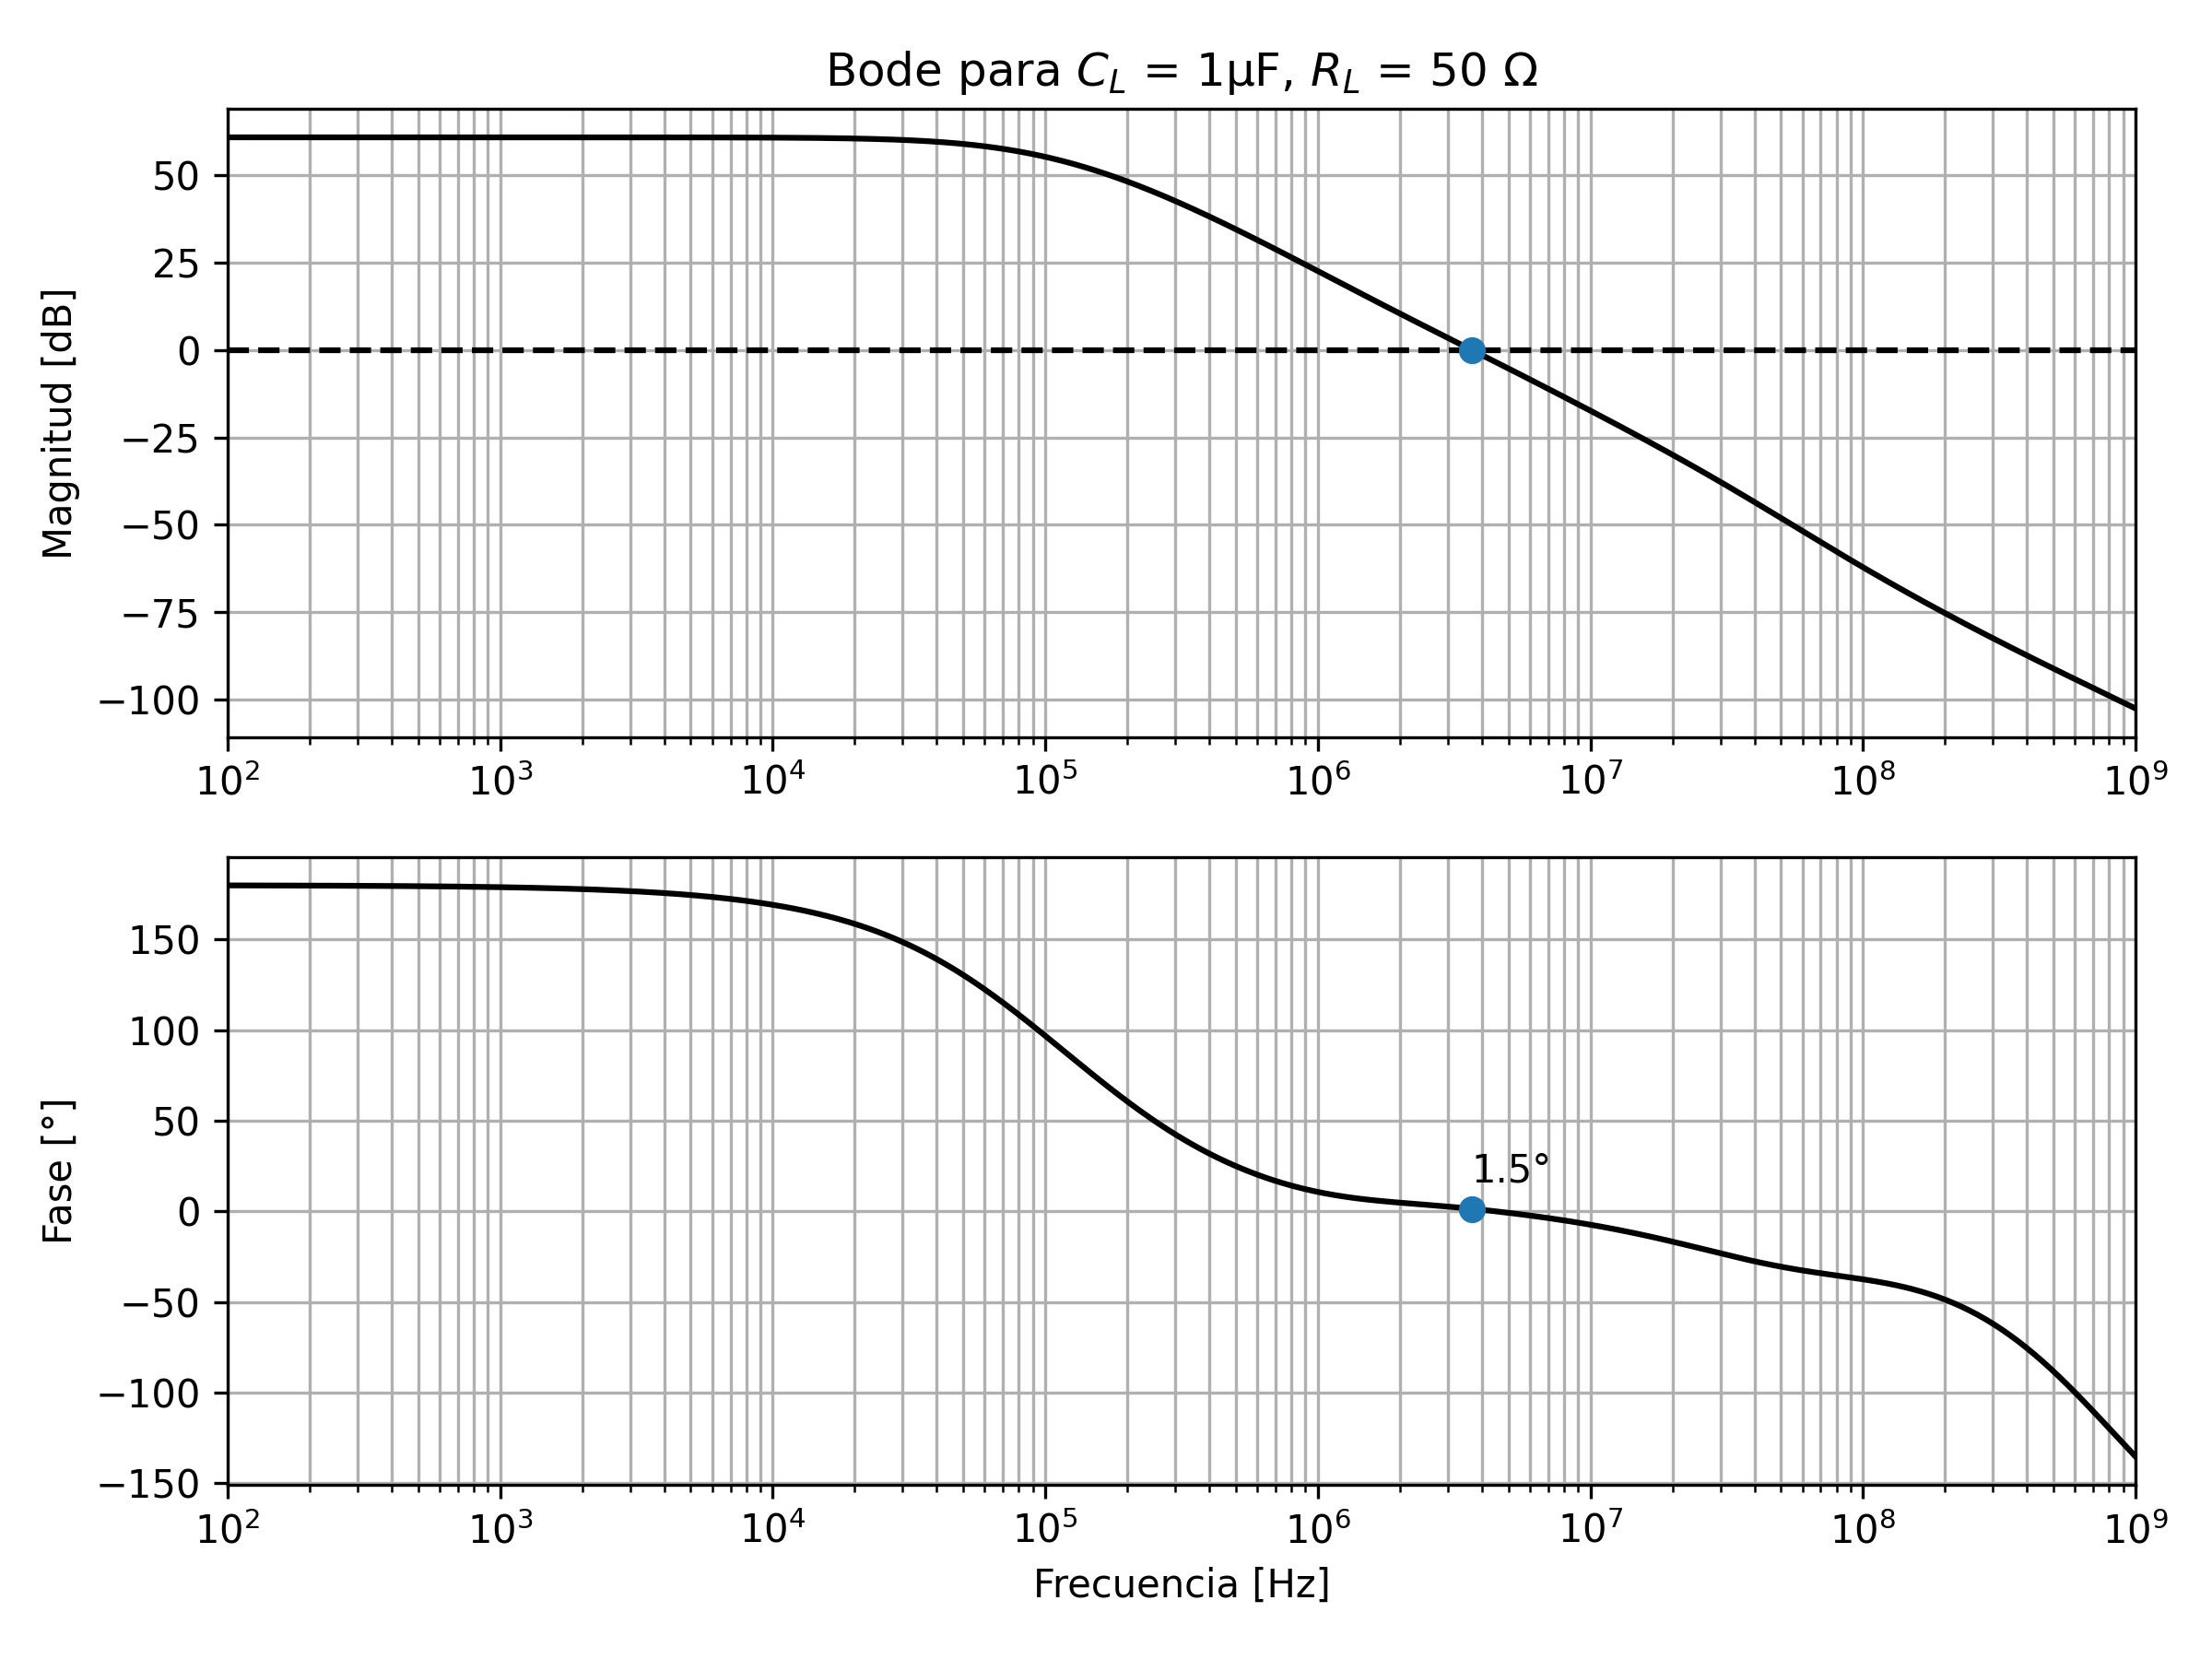
\includegraphics[width=0.9\linewidth]{img/Lazo de tensión/LT sin compensar.png}
    \caption{Lazo de tensión sin compensar para $R_L = 50 \Omega$ y $C_L = \SI{1}{\micro \farad}$}
    \label{fig:LT sin compensar}
\end{figure}

Se observa que el margen de fase es muy chico, por lo que el circuito está al borde de la inestabilidad. Por otro lado, se observa que el polo dominante está a aproximadamente \SI{100}{\kilo \hertz}. Analizando el circuito, puede intuirse que el polo dominante se debe al nodo de salida del par diferencial, ya que este es el nodo con más capacitores unidos. Habrá entonces una capacidad y una resistencia equivalentes entre el nodo y tierra, lo que implicaría un valor para el polo dominante de $p = \frac{1}{2\pi R_N C_N}$. Por lo tanto, puede agregarse un capacitor entre el nodo y tierra, el cual se sumaría al valor de la capacidad ya presente en el nodo y reduciría la frecuencia del polo dominante. 

Para estimar un valor para el capacitor de compensación, puede calcularse de forma aproximada la capacidad equivalente del nodo $C_N$ usando la técnica de reflexión de Miller. 

\begin{equation}
    C_N = C_{\mu1} + C_{\mu2} + C_{\mu3}\cdot (1 + g_{m3} \, r_{\pi4}) = \SI{22}{\pico \farad}
\end{equation}

En esta ecuación los valores de la resistencia, transconductancia y capacidades se obtuvieron de una simulación \texttt{.op} de \texttt{LTSpice}. Cabe aclarar que este resultado es solo una aproximación, ya que se hicieron varias simplificaciones, como que la ganancia base-colector de Q3 era 1 y que en frecuencia el capacitor $C_L$ es un cortocircuito.

En cualquier caso, se necesita disminuir el valor del polo dominante en por lo menos 3 décadas, de forma tal de disminuir la frecuencia de cruce por 0 dB y llevarla a una donde todavía haya suficiente fase. Por lo tanto, debe elegirse un capacitor 3 órdenes de magnitud superior a $C_N$. Eso da un capacitor del orden de las decenas de \SI{}{\nano \farad}, pero es preferible usar uno de un orden de magnitud mayor para hacer al circuito robusto ante posibles variaciones en los valores de los componentes. De esta forma, se probaron valores comerciales para capacitores entre \SI{100}{\nano \farad} y \SI{1}{\micro \farad} y se eligió un capacitor de \SI{330}{\nano \farad}.

El diagrama de Bode del lazo de tensión compensado se muestra en la \autoref{fig:LT compensado}

\begin{figure}
    \centering
    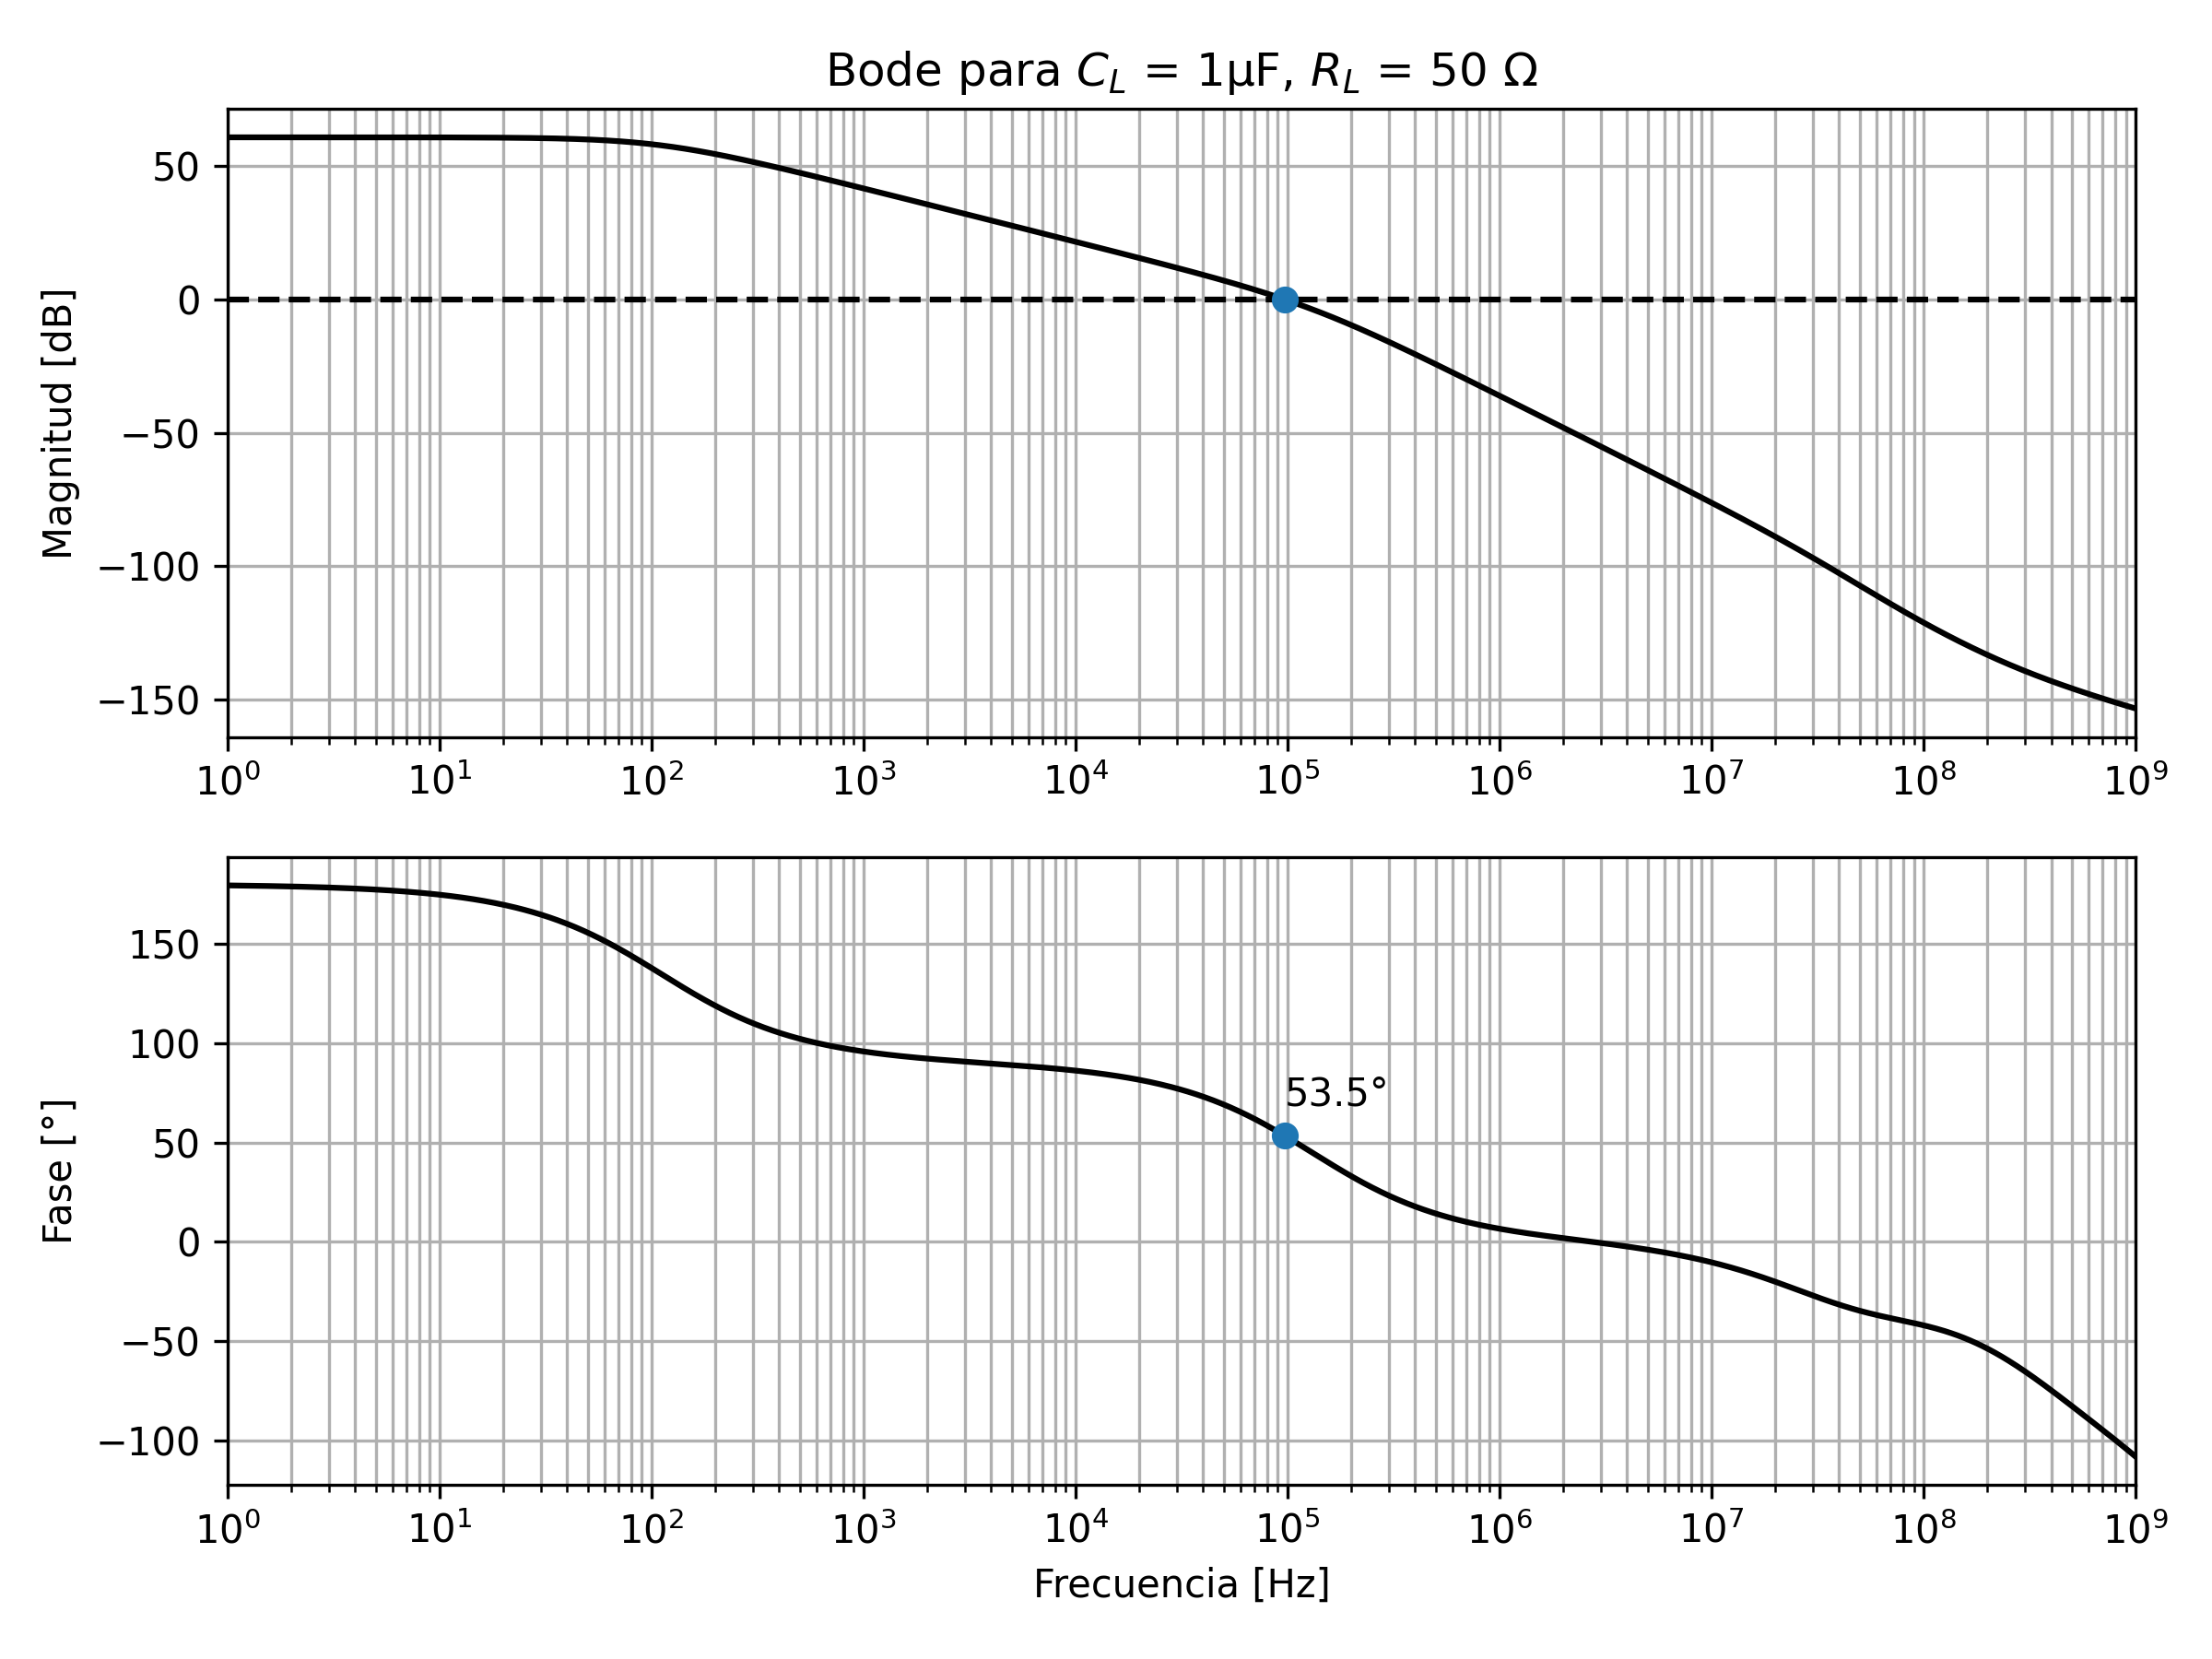
\includegraphics[width=0.9\linewidth]{img/Lazo de tensión/LT compensado.png}
    \caption{Diagrama de Bode del lazo de tensión compensado}
    \label{fig:LT compensado}
\end{figure}

Para apreciar el efecto de la compensación, se simularon las respuestas al escalón del lazo sin compensar y el compensado.

\begin{figure}[H]
    \centering
    
    \begin{subfigure}{0.9\textwidth}
        \centering
        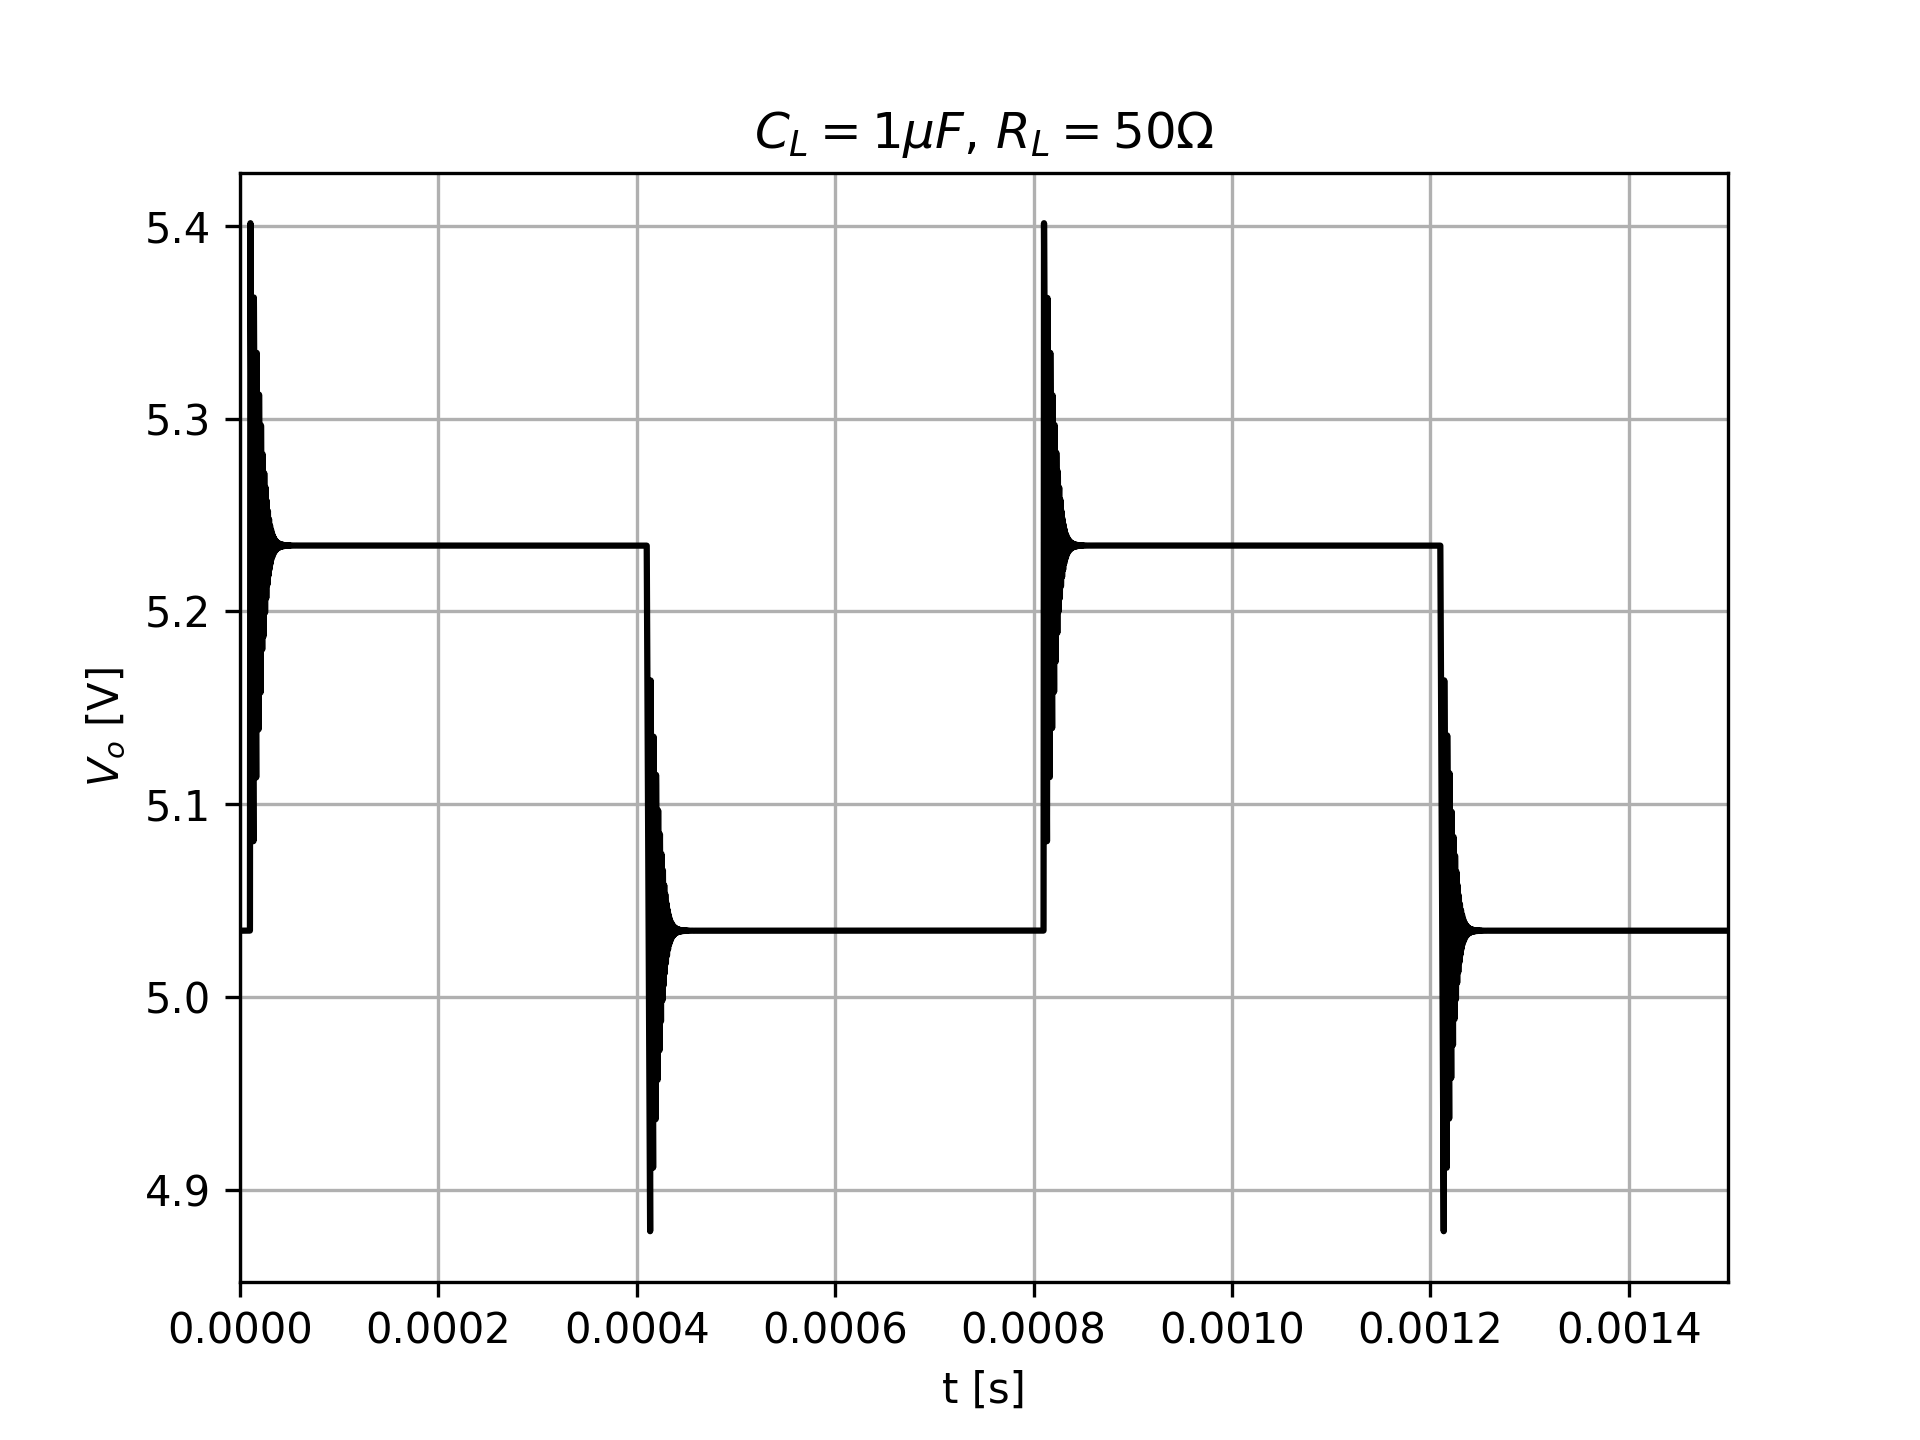
\includegraphics[width=\textwidth]{img/Lazo de tensión/Rta al escalon(sin compensar).png}
        \caption{Respuesta al escalón sin compensar}
        \label{Rta al escalón sin compensar}
    \end{subfigure}
    
    \vspace{0.3cm}
    
    \begin{subfigure}{0.9\textwidth}
        \centering
        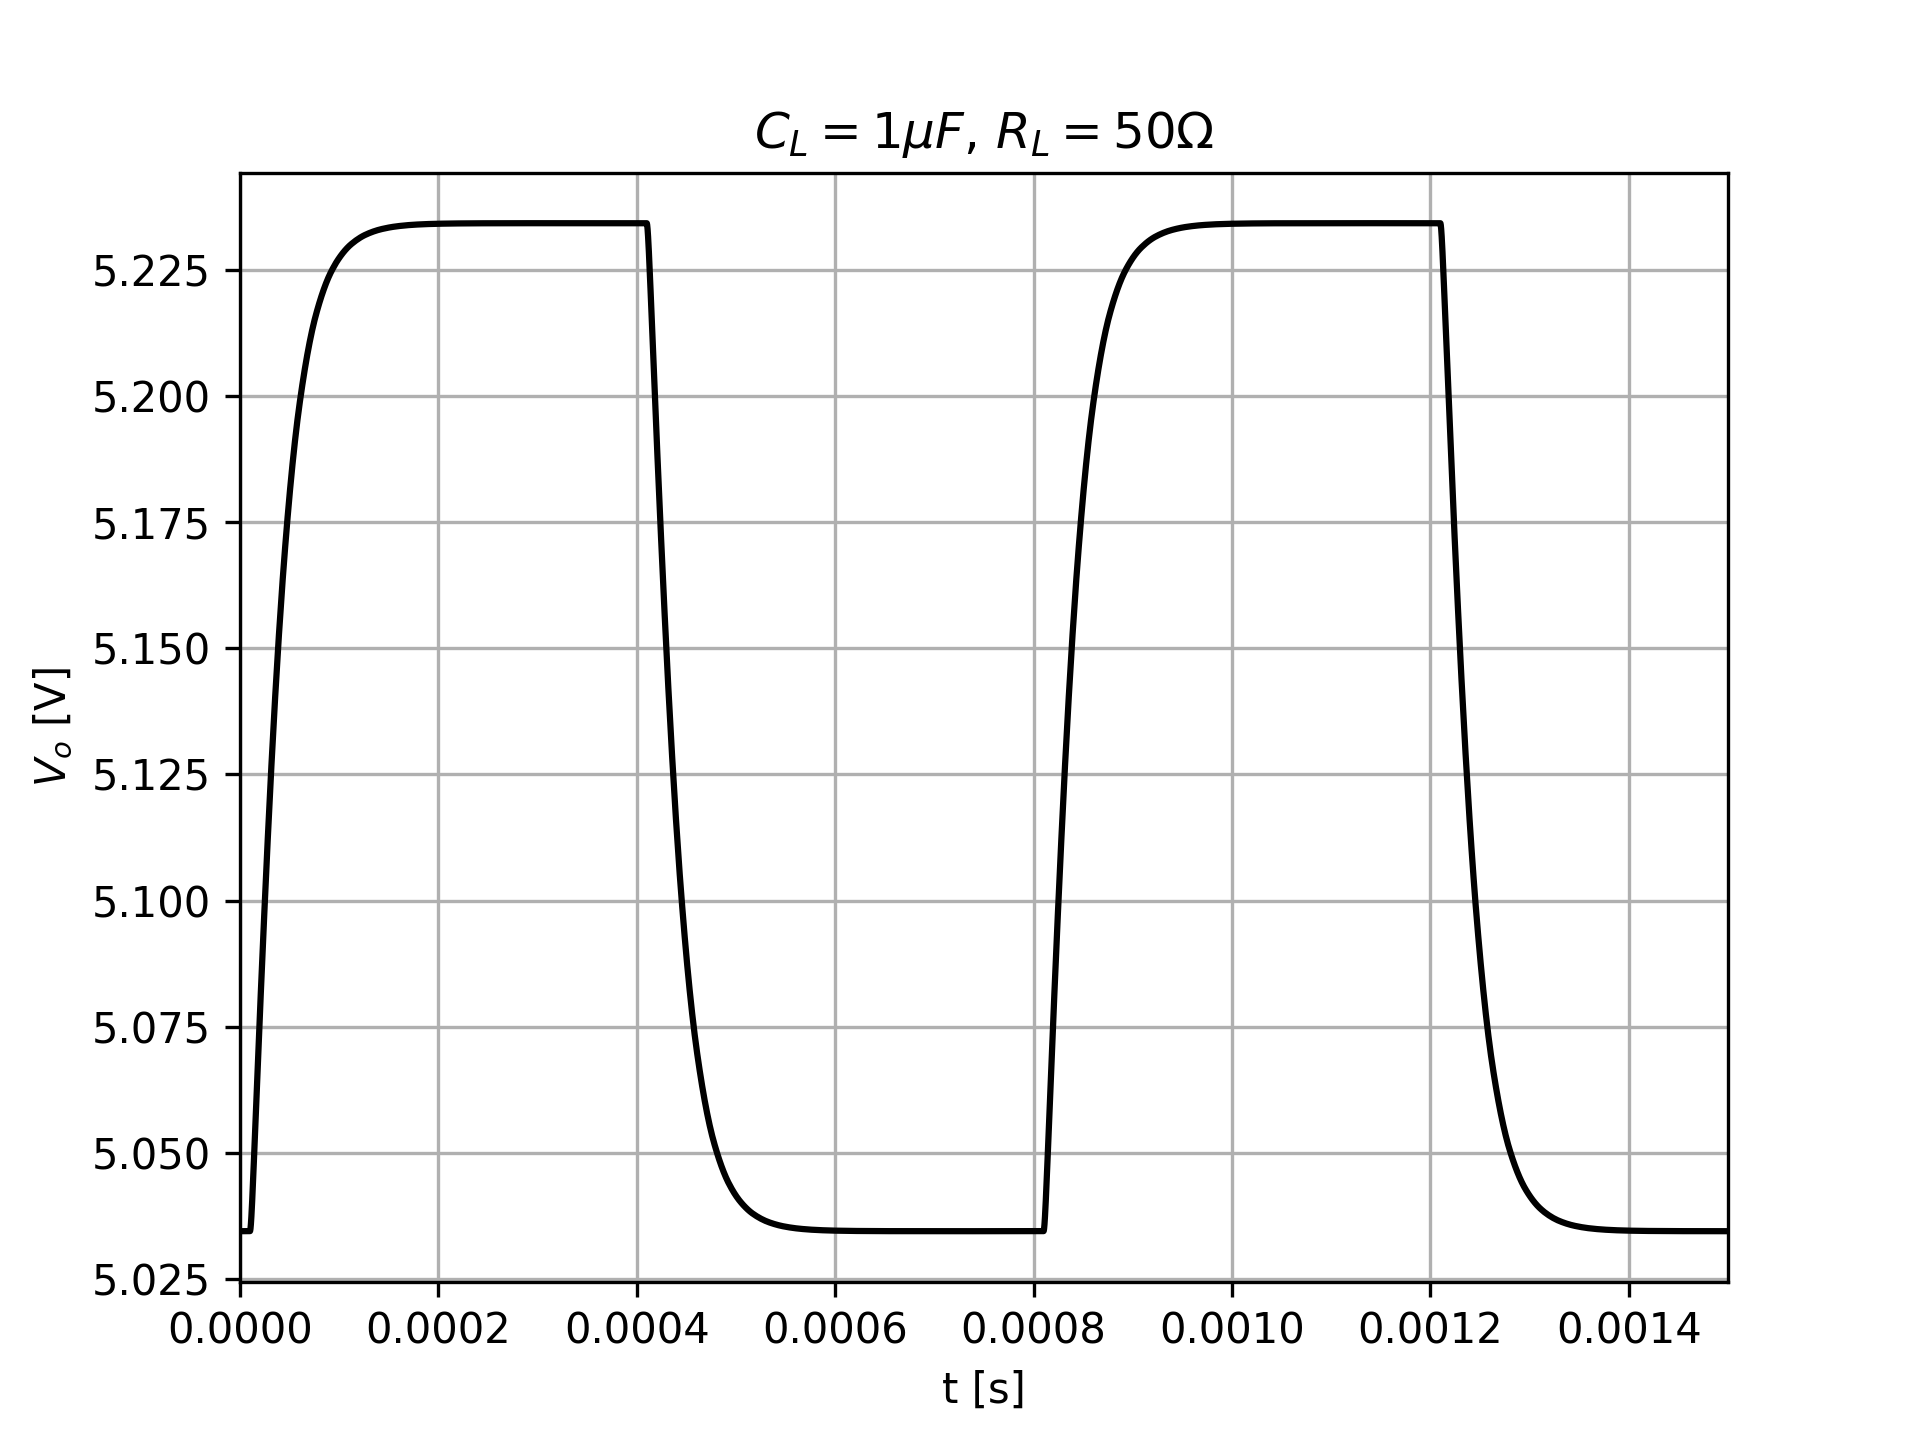
\includegraphics[width=\textwidth]{img/Lazo de tensión/Rta al escalon(compensada).png}
        \caption{Respuesta al escalón compensada}
        \label{Rta al escalon compensada}
    \end{subfigure}
    
    \caption{Respuestas al escalón}
\end{figure}

